\chapter{TINJAUAN PUSTAKA}
\label{chap:tinjauanpustaka}



\section{Hasil penelitian/perancangan terdahulu}
Dalam penelitian ini, penulis merujuk pada beberapa studi sebelumnya yang relevan. Penelitian-penelitian tersebut memiliki hubungan dengan topik yang sedang diteliti, sehingga dapat digunakan sebagai dasar untuk penelitian ini.

\subsection{\emph{Autonomous Thermal Vision Robotic System for Victims Recognition}}

Penelitian oleh Cruz Ulloa mengembangkan robot berkaki empat (\emph{quadruped-legged}) menggunakan \emph{Unitree A1} yang dilengkapi dengan kamera termal \emph{Optris Pi640}. Robot ini dirancang untuk mendeteksi korban dalam misi pencarian dan penyelamatan di lingkungan pasca-bencana, dengan memanfaatkan citra termal yang dianalisis menggunakan algoritma \emph{Convolutional Neural Network (CNN)}. Hasil penelitian menunjukkan bahwa sistem ini mampu mencapai akurasi deteksi lebih dari 90\% dalam kondisi ekstrem, seperti lingkungan minim cahaya atau area yang dipenuhi puing bangunan. Robot ini beroperasi secara \emph{teleoperated} dan mampu menjelajah medan yang tidak rata, sehingga sangat membantu tim pencarian dalam menemukan korban yang terperangkap di lokasi bencana \cite{Cruz2021}. Sistem robot dibangun dengan menggunakan \emph{Robot Operating System (ROS) 1 Melodic}, seperti pada gambar \ref{fig:Quadruped dengan kamera termal untuk deteksi korban}

\begin{figure} [H] \centering
  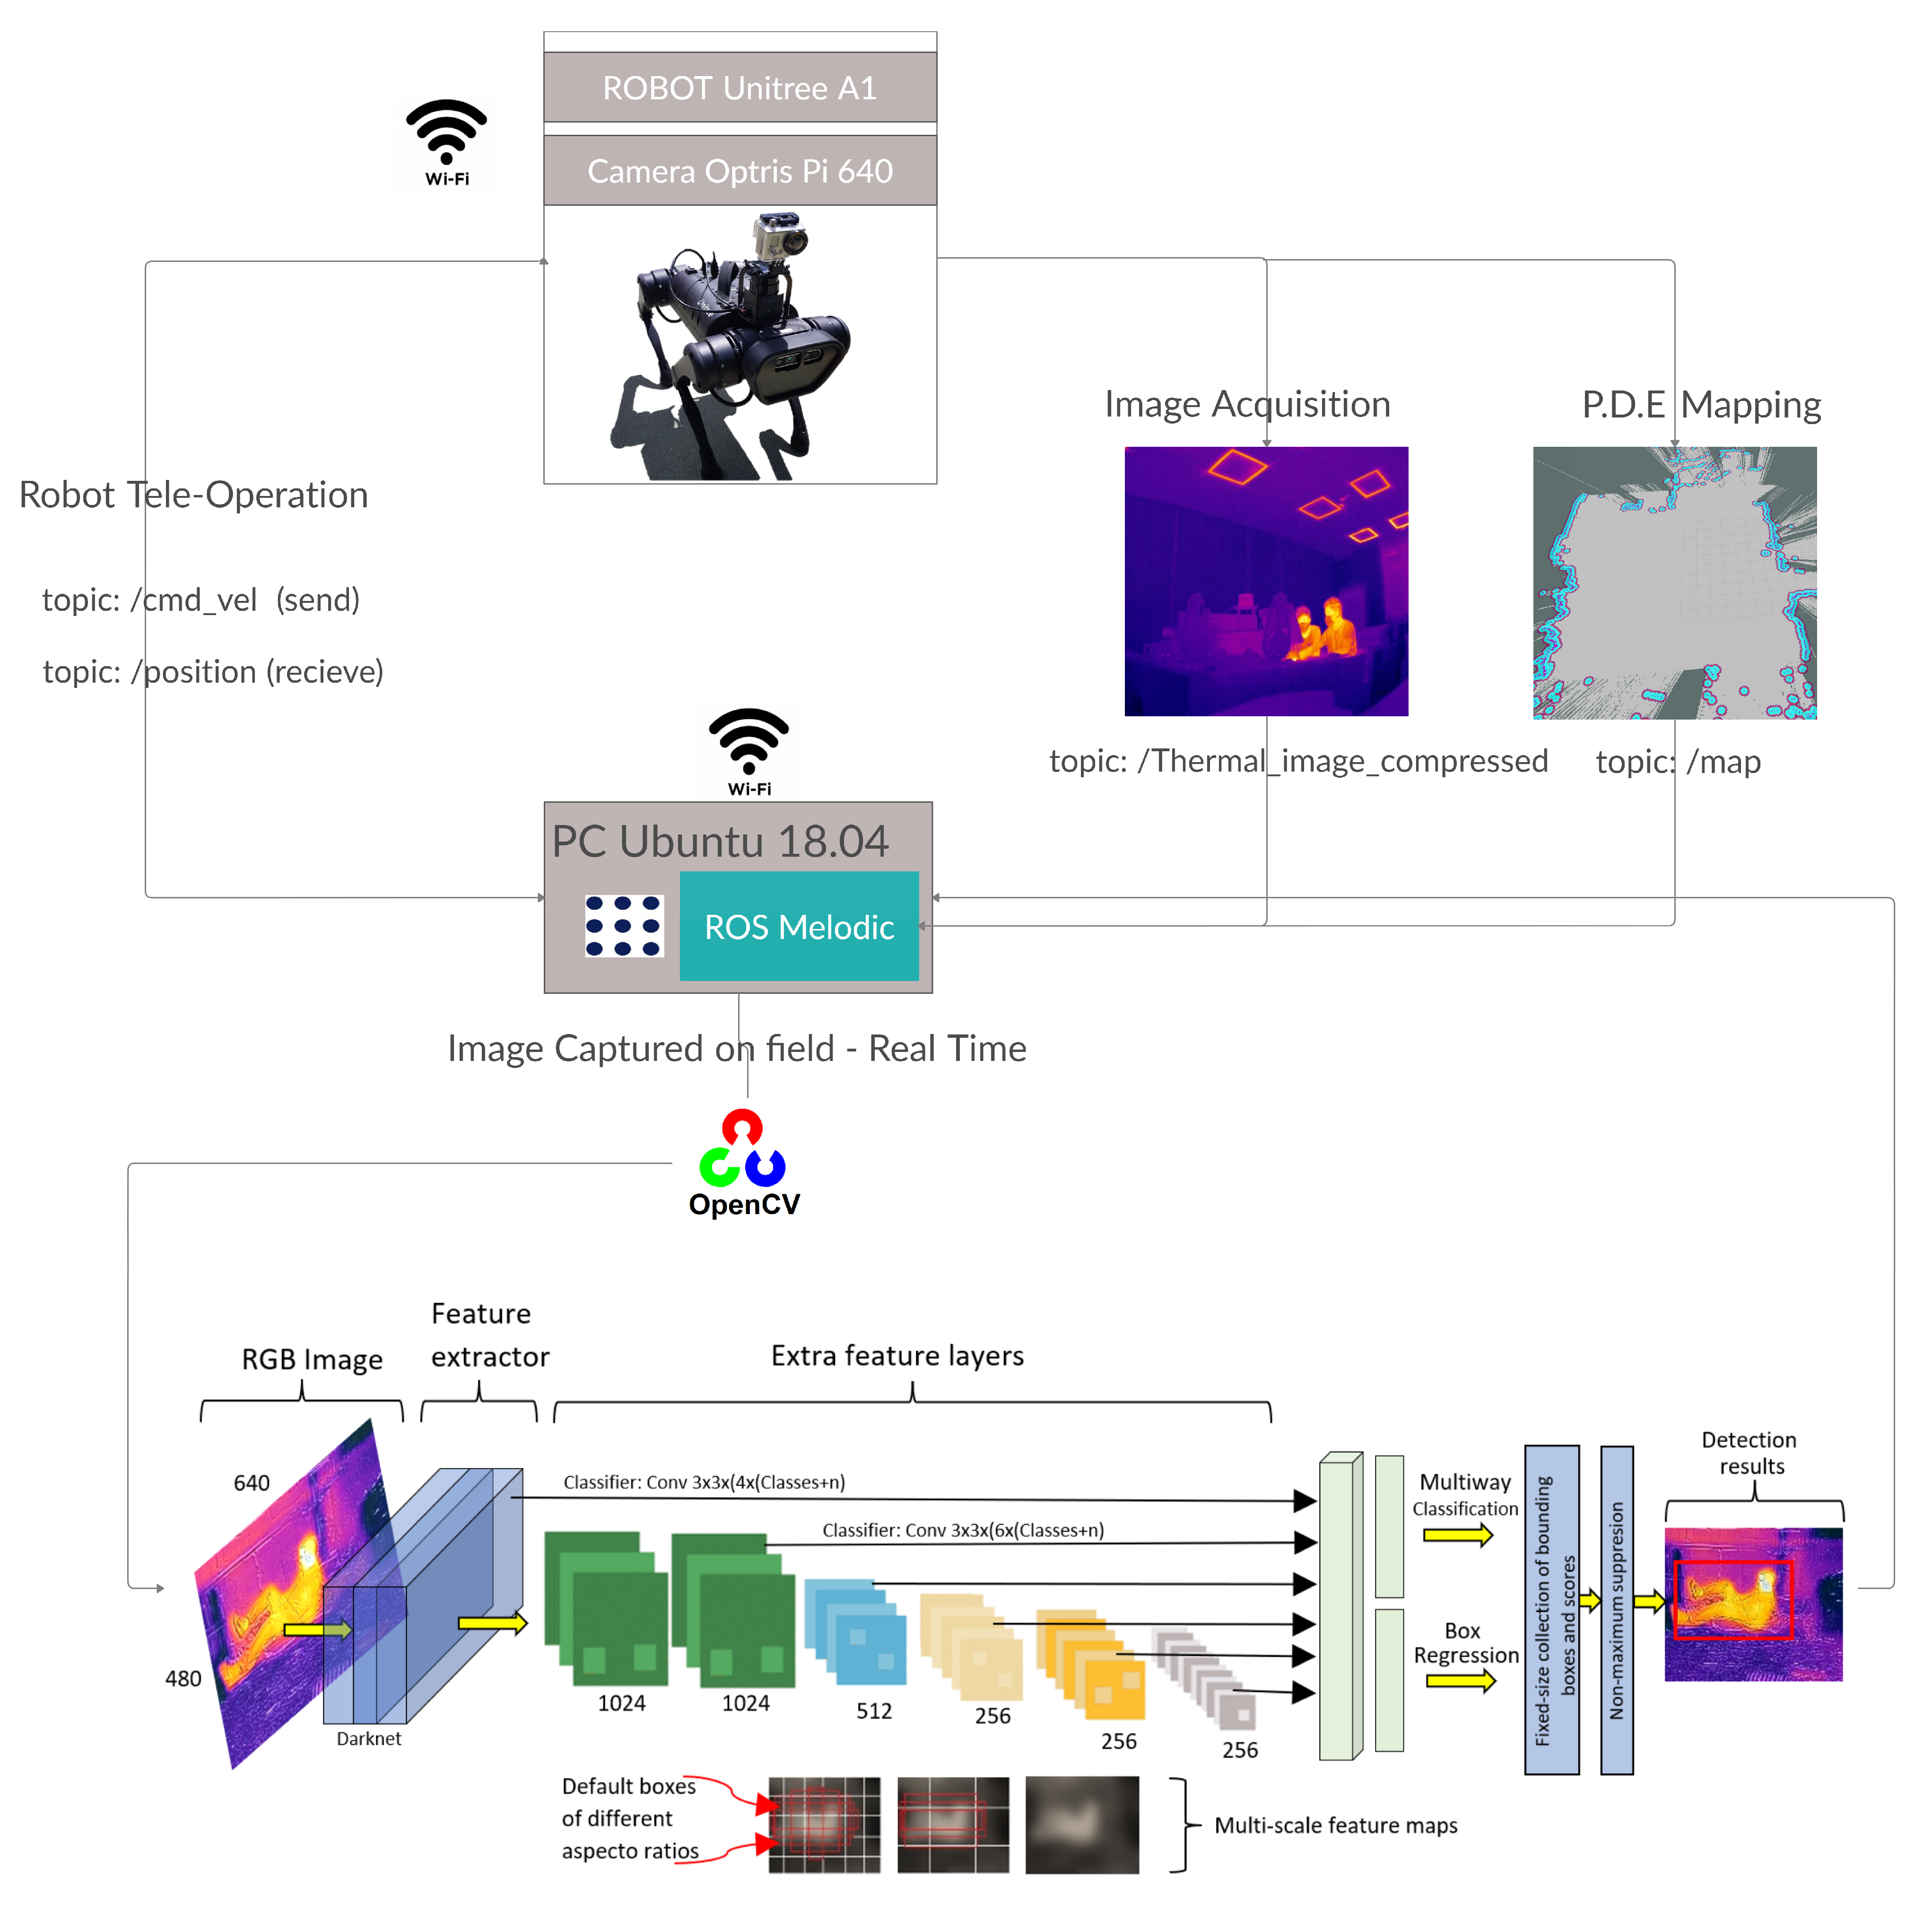
\includegraphics[scale=0.057]{gambar/bab2/unitreea1.png}
  \caption{\emph{Quadruped robot} dengan kamera termal untuk deteksi korban}
  \label{fig:Quadruped  dengan kamera termal untuk deteksi korban}
  \footnotesize{\textbf{Sumber:} Cruz Ulloa (2021)}
\end{figure}

Penelitian ini memiliki kesamaan dengan topik yang sedang dikembangkan, yaitu penggunaan robot \emph{quadruped} dan kamera termal untuk memberikan estimasi posisi objek dalam peta, menjadikannya sangat relevan dengan pendekatan yang sedang dirancang.



\subsection{\emph{Image Processing Technique Applied to Electrical
Substations Based on Drones With Thermal Vision
for Predictive Maintenance}}
Penelitian ini mengusulkan penggunaan \emph{VANT} (Vehículo Aéreo No Tripulado) atau drone, yang dilengkapi dengan dua jenis kamera: \emph{kamera tradisional} untuk menangkap gambar visual dan \emph{kamera termografik} untuk memperoleh gambar inframerah yang dapat menunjukkan suhu komponen di gardu induk. Drone ini dilengkapi dengan sistem navigasi dan pengendalian yang memungkinkan operasi otonom di sekitar gardu induk. Data gambar yang diambil oleh drone diproses menggunakan teknik \emph{image processing} untuk mengidentifikasi \emph{hot spots} atau titik panas pada komponen gardu induk.

\begin{figure} [H] \centering
  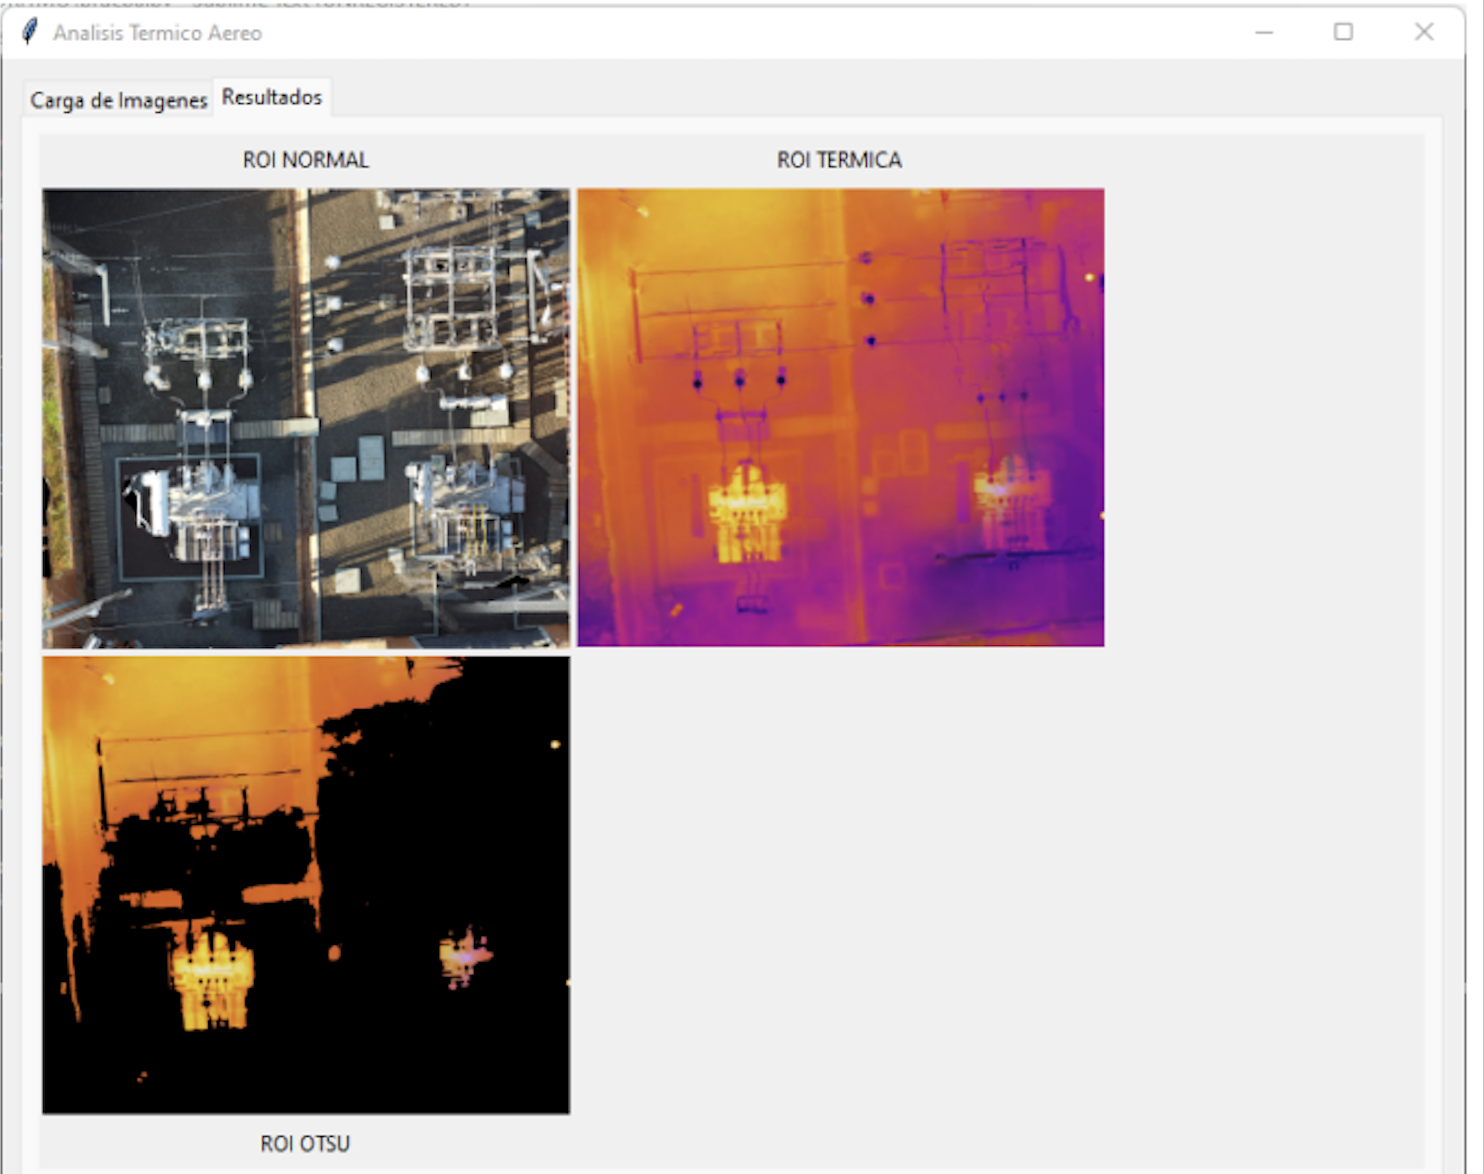
\includegraphics[scale=0.64]{gambar/bab2/drone.png}
  \caption{Drone dengan kamera termal untuk pemantauan gardu induk}
  \label{fig:Drone dengan kamera termal untuk pemantauan gardu induk}
  \footnotesize{\textbf{Sumber:} Prieto et al. (2022)}
\end{figure}

Hasil analisis ini dapat digunakan untuk memprediksi potensi kerusakan pada komponen dan mengambil tindakan pencegahan yang diperlukan. Penelitian ini menunjukkan bahwa penggunaan drone dengan kamera termal dapat meningkatkan efisiensi dan akurasi dalam pemantauan gardu induk, serta meminimalkan risiko keselamatan bagi petugas yang harus melakukan inspeksi langsung di lokasi gardu \cite{Prieto2022}. Penelitian ini memiliki kesamaan dengan topik kami yang juga menggunakan kamera termal untuk pemantauan komponen gardu listrik.

\section{Teori/Konsep Dasar}
Subbab ini membahas berbagai teori dan konsep dasar yang menjadi landasan dalam penyusunan tugas akhir. Penjelasan dalam bab ini mencakup berbagai teori yang relevan dan digunakan dalam pelaksanaan penelitian.

\subsection{Gardu Listrik}
\sloppy
Gardu listrik merupakan salah satu komponen vital dalam sistem kelistrikan yang berfungsi sebagai titik penghubung antara pembangkit listrik dan jaringan distribusi. Melalui gardu listrik, aliran energi listrik dapat diatur dan dialirkan secara efisien dari sumber pembangkit menuju konsumen akhir \cite{stevenson1994power}. Proses transmisi dan distribusi energi listrik tidak dapat dilakukan secara aman dan terkontrol tanpa adanya gardu listrik. Secara umum, terdapat beberapa jenis gardu listrik, antara lain gardu induk dan gardu pembangkit. Gardu induk memiliki fungsi utama untuk menurunkan tegangan listrik dari tingkat tinggi, yang digunakan dalam proses transmisi, menjadi tegangan menengah atau rendah agar aman untuk digunakan oleh konsumen \cite. Gardu ini umumnya terletak di antara pembangkit dan kawasan konsumen, baik permukiman maupun kawasan industri.

Sementara itu, gardu pembangkit merupakan fasilitas yang berada di dekat sumber energi primer, seperti pembangkit listrik tenaga air (PLTA), pembangkit listrik tenaga uap (PLTU), atau jenis pembangkit lainnya. Gardu ini berfungsi untuk menyalurkan energi listrik yang dihasilkan dari proses konversi energi primer ke jaringan transmisi. Untuk mendukung fungsinya, gardu listrik dilengkapi dengan berbagai peralatan kelistrikan, seperti transformator, pemutus sirkuit, dan isolator untuk menjamin keandalan sistem. Keandalan gardu listrik sangat berpengaruh terhadap kualitas dan kontinuitas pasokan energi listrik \cite{gonen2016electric}.

\subsubsection{2.2.1.1 Transformator}
Transformator merupakan salah satu komponen utama dalam gardu listrik yang berfungsi untuk mengubah tingkat tegangan sesuai kebutuhan dalam proses transmisi maupun distribusi energi listrik. Salah satu jenis transformator yang umum pada gardu listrik adalah transformator daya. Transformator daya digunakan untuk menyesuaikan tegangan agar sesuai dengan kebutuhan sistem, sekaligus meminimalkan rugi-rugi daya selama proses transmisi jarak jauh. Berdasarkan fungsinya, transformator daya dibedakan menjadi dua jenis, yaitu transformator \emph{step-up} dan transformator \emph{step-down}  Transformator \emph{step-up} digunakan di sisi pembangkit untuk menaikkan tegangan listrik ke tingkat yang lebih tinggi agar transmisi lebih efisien dan rugi daya berkurang, sedangkan transformator \emph{step-down} digunakan di sisi distribusi untuk menurunkan tegangan ke tingkat yang lebih rendah sehingga aman digunakan oleh konsumen . Transformator daya biasanya dirancang untuk beroperasi pada suhu maksimum sekitar 105\textdegree{}C hingga 110\textdegree{}C, tergantung pada kelas isolasi termal yang digunakan, seperti kelas A, B, atau F \cite{stevenson1994power}.

\subsubsection{2.2.1.2 \emph{Arrester}}
\emph{Arrester}, atau \emph{lightning arrester}, merupakan perangkat pelindung dalam sistem kelistrikan yang berfungsi untuk mengamankan peralatan dari lonjakan tegangan akibat sambaran petir atau gangguan tegangan lebih sesaat. \emph{Arrester} bekerja dengan cara mengalihkan arus lebih tersebut langsung ke \emph{ground}, sehingga mencegah terjadinya kerusakan pada peralatan penting seperti transformator, pemutus sirkuit, dan komponen lainnya di gardu listrik. Pemeliharaan rutin terhadap \emph{arrester} sangat penting dilakukan untuk memastikan performanya tetap optimal. Salah satu parameter penting yang harus dipantau adalah suhu operasi perangkat. Umumnya, \emph{arrester} dirancang untuk beroperasi pada suhu lingkungan antara -40\textdegree{}C hingga 60\textdegree{}C. Jika suhu operasional melebihi batas maksimum tersebut, maka dapat terjadi kerusakan permanen pada komponen internal arrester yang berakibat pada menurunnya efektivitas perlindungan sistem secara keseluruhan \cite{Kartika2022}.

\subsubsection{2.2.1.3 Disconnector}
\emph{Disconnector} merupakan perangkat yang berfungsi untuk memisahkan suatu bagian dari sistem kelistrikan guna keperluan pemeliharaan atau perbaikan, tanpa memengaruhi bagian lain dari jaringan. Pemeliharaan serta pengujian secara berkala terhadap \emph{disconnector} sangat krusial untuk memastikan bahwa perangkat ini dapat berfungsi secara optimal saat dibutuhkan. Suhu operasi \emph{disconnector} umumnya berada dalam kisaran 20°C hingga 40°C. Namun, apabila suhu meningkat melebihi 85°C, dapat terjadi overheating yang berpotensi menyebabkan kegagalan fungsi \cite{Henriana2022}.


\subsubsection{2.2.1.4 Busbar}
\emph{Busbar} adalah komponen dalam gardu listrik yang berfungsi sebagai penghubung antara berbagai peralatan listrik. \emph{Busbar} memungkinkan distribusi arus listrik yang efisien dan aman di dalam gardu. \emph{Busbar} biasanya terbuat dari bahan konduktif yang baik, seperti tembaga atau aluminium, dan dirancang untuk menampung arus listrik dalam jumlah besar. Pemeliharaan dan pengujian \emph{busbar} secara rutin diperlukan untuk mencegah kerusakan dan memastikan keandalan sistem distribusi listrik. Suhu operasi \emph{busbar} dapat bervariasi, tetapi umumnya tidak boleh melebihi 90°C untuk mencegah overheating yang dapat merusak isolasi dan struktur busbar itu sendiri \cite{Telaumbanua2024}.

\subsubsection{2.2.1.5 Isolator}
\emph{Isolator} adalah perangkat yang berfungsi untuk memisahkan bagian dari sistem kelistrikan, sehingga mencegah arus listrik mengalir ke bagian yang tidak diinginkan. \emph{Isolator} digunakan untuk menjaga keamanan dan keandalan sistem kelistrikan, terutama saat pemeliharaan dilakukan. \emph{Isolator} dirancang untuk menahan tegangan tinggi dan memiliki karakteristik dielektrik yang baik. Pemeliharaan \emph{isolator} juga penting untuk memastikan bahwa tidak ada kebocoran arus yang dapat menyebabkan kerusakan pada peralatan lainnya. Suhu operasi \emph{isolator} biasanya berkisar antara -30°C hingga 50°C, dan overheating dapat terjadi jika suhu melebihi 70°C, yang dapat mengakibatkan kerusakan pada material isolasi \cite{Moreno2017}.

\subsubsection{2.2.1.6 Pemutus Sirkuit (\emph{Circuit Breaker})}
\emph{Pemutus sirkuit} adalah perangkat yang berfungsi untuk melindungi sistem kelistrikan dari arus lebih (\emph{overcurrent}) dan hubung singkat (\emph{short circuit}). \emph{Pemutus sirkuit} dapat secara otomatis memutuskan aliran listrik ketika terdeteksi adanya gangguan, sehingga mencegah kerusakan pada peralatan dan menjaga keselamatan sistem. Terdapat berbagai jenis \emph{pemutus sirkuit}, termasuk \emph{pemutus sirkuit otomatis} (\emph{automatic circuit breaker}) dan \emph{pemutus sirkuit manual} (\emph{manual circuit breaker}), yang masing-masing memiliki aplikasi dan karakteristik yang berbeda Pemeliharaan dan pengujian berkala terhadap \emph{pemutus sirkuit} sangat penting untuk memastikan bahwa perangkat ini berfungsi dengan baik saat dibutuhkan. Suhu operasi \emph{pemutus sirkuit} biasanya berkisar antara -25°C hingga 55°C, dan overheating dapat terjadi jika suhu melebihi 85°C, yang dapat menyebabkan kerusakan pada mekanisme pemutus \cite{Ilomets2020}.

\subsection{DeepRobotics Jueying X30 Pro}
DeepRobotics Jueying X30 Pro adalah robot berkaki empat (\textit{quadruped}) generasi terbaru yang dikembangkan oleh perusahaan teknologi robotik DeepRobotics di Tiongkok. Dirancang untuk berbagai aplikasi industri seperti inspeksi fasilitas, penyelamatan darurat, eksplorasi lingkungan ekstrem, serta pemantauan di berbagai medan, robot ini mengintegrasikan teknologi berbagai sensor untuk navigasi dan persepsi lingkungan. Dalam mendukung navigasi dan pemetaan lingkungan, X30 Pro dilengkapi dengan empat sensor LiDAR 360° Livox, dua di bagian depan dan dua di bagian belakang. Selain itu, X30 Pro dilengkapi dengan IMU (\textit{Inertial Measurement Unit}) Yesense YIS100-V, yang menggabungkan akselerometer dan giroskop untuk mengukur percepatan linear dan kecepatan sudut. Dengan desain industrial Jueying X30 Pro mampu bergerak secara cepat dan stabil di berbagai jenis permukaan. Kemampuan tersebut didukung oleh integrasi teknologi persepsi \emph{multimodal} dan sistem kendali gerak adaptif, sehingga memungkinkan navigasi otonom dalam kondisi lingkungan yang kompleks. Spesifikasi teknis utama dari Jueying X30 Pro ditampilkan pada Tabel~\ref{tab:spesifikasiX30}.


\begin{table}[H]
	\centering
	\caption{Spesifikasi Teknis Deep Robotics X30}
	\label{tab:spesifikasiX30}
	\renewcommand{\arraystretch}{1.2}
	\begin{tabular}{|p{5.5cm}|p{7cm}|}
		\hline
		\textbf{Parameter}            & \textbf{Spesifikasi}                                              \\
		\hline
		Dimensi (P × L × T)           & 1000 mm × 585 mm × 470 mm                                         \\
		\hline
		Bobot (berat bersih)          & 56--59 kg                                                         \\
		\hline
		Kecepatan Maksimal            & 4 m/s                                                             \\
		\hline
		Kemampuan Menanjak            & Hingga 45\textdegree{} (termasuk tangga terbuka)                  \\
		\hline
		Ketinggian Rintangan Maksimal & $\geq$ 20 cm                                                      \\
		\hline
		Rentang Suhu Operasional      & --20\textdegree{}C hingga +55\textdegree{}C                       \\
		\hline
		Perlindungan Lingkungan       & IP67 (tahan air dan debu)                                         \\
		\hline
		Daya Tahan Baterai            & 2,5--4 jam (dengan beban penuh)                                   \\
		\hline
		Sistem Pengisian Daya         & Pengisian otomatis (\emph{auto-charging}), \emph{manual charging} \\
		\hline
		Antarmuka Komunikasi          & Ethernet, USB 2.0/3.0, dan Wi-Fi                                  \\
		\hline
	\end{tabular}
	\footnotesize\\ \textbf{Sumber:} DEEP Robotics (2023)
\end{table}


Untuk mendukung operasi otonom dan efisien, \emph{DeepRobotics Jueying X30 Pro} dilengkapi dengan tiga unit komputer onboard yang masing-masing bertanggung jawab atas fungsi gerak (\emph{motion}), persepsi (\emph{perception}), dan navigasi (\emph{navigation}). Arsitektur ini memungkinkan pemrosesan paralel dan spesialisasi tugas, meningkatkan kinerja robot dalam lingkungan yang kompleks dan dinamis. Ketiga komputer ini terhubung melalui Ethernet seperti pada Gambar \ref{fig:network_architecture_x30pro}.


\begin{figure}[H]
  \centering
  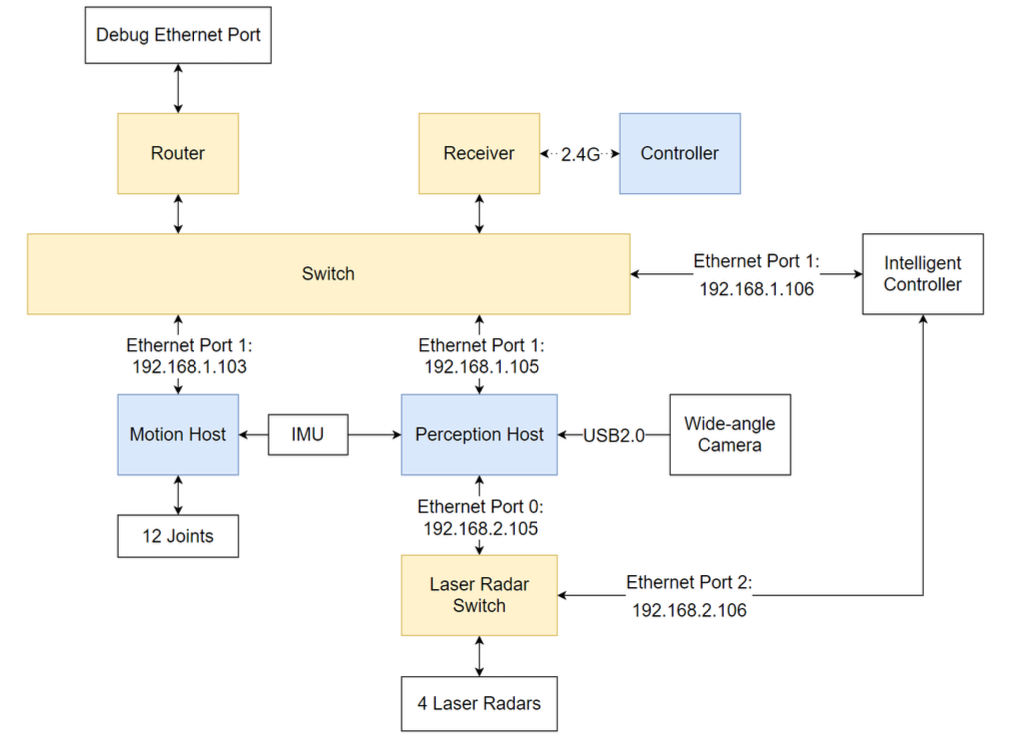
\includegraphics[width=0.65\textwidth]{gambar/bab2/network-x30.png}
  \caption{Arsitektur Jaringan Internal \emph{DeepRobotics Jueying X30 Pro}}
  \label{fig:network_architecture_x30pro}
  \footnotesize{\textbf{Sumber:} DeepRobotics (2023)}
\end{figure}


Arsitektur modular ini tidak hanya meningkatkan efisiensi operasional tetapi juga memudahkan integrasi dengan sistem eksternal dan pembaruan perangkat lunak. Robot ini menggunakan \emph{Robot Operating System (ROS) Noetic Ninjameys} dan dijalankan menggunakan sistem operasi Ubuntu 20.04, yang semakin memperluas potensi integrasi dan pengembangan aplikasi berbasis \emph{open-source}.


\subsection{Hikvision HM-TD5528T-15/W}

Hikvision HM-TD5528T-15/W adalah kamera termal cerdas untuk pemantauan area kritis seperti gardu distribusi, industri, dan zona rawan kebakaran. Perangkat ini menggabungkan sensor termal presisi tinggi, deteksi suhu real-time, serta kemampuan mendeteksi api dan asap secara simultan. Dengan desain tahan cuaca ekstrem, kamera ini ideal untuk pengawasan luar ruang jangka panjang. Rincian spesifikasi utama ditampilkan pada Tabel~\ref{tab:spesifikasiHikvision}.

\begin{table}[H]
    \centering
    \caption{Spesifikasi Teknis Hikvision HM-TD5528T-15/W}
    \label{tab:spesifikasiHikvision}
    \renewcommand{\arraystretch}{1.2}
    \begin{tabular}{|p{6cm}|p{7.5cm}|}
        \hline
        \textbf{Parameter} & \textbf{Spesifikasi} \\
        \hline
        Sensor Termal & Vanadium Oxide Uncooled FPA \\
        \hline
        Resolusi & \(256 \times 192\) piksel \\
        \hline
        Pixel Pitch & \(12~\mu\mathrm{m}\) \\
        \hline
        Rentang Spektral & \(8 - 14~\mu\mathrm{m}\) \\
        \hline
        NETD & \(\leq 35~\text{mK}\) @ \(25^\circ\text{C}\), F1.0 \\
        \hline
        Panjang Fokus & 15 mm \\
        \hline
        Field of View & \(11.69^\circ \times 8.78^\circ\) \\
        \hline
        IFOV & \(0.8~\text{mrad}\) \\
        \hline
        Deteksi Kendaraan & 1917 m (deteksi), 240 m (identifikasi) \\
        \hline
        Pengukuran Suhu & Titik, area, garis; akurasi \(\pm 2^\circ\text{C}\) atau \(\pm 2\%\) \\
        \hline
        Protokol Jaringan & RTSP, ISAPI, ONVIF, SDK \\
        \hline
        Perlindungan & IP67, tahan \(-40^\circ\text{C}\) s.d. \(70^\circ\text{C}\), petir 6000 V \\
        \hline
    \end{tabular}
    \footnotesize\\ \textbf{Sumber:} Hikvision Datasheet (2025)
\end{table}

Dengan kemampuan deteksi suhu tinggi dan cakupan jarak jauh, HM-TD5528T-15/W ideal untuk pemantauan kondisi trafo, koneksi kabel, dan komponen gardu lainnya. Dukungan RTSP dan ISAPI memudahkan integrasi dengan software berbasis ROS dan Website. 

\subsection{\emph{Robot Operating System (ROS)}}
\emph{Robot Operating System (ROS)} adalah \emph{framework} perangkat lunak \emph{open-source} yang dirancang untuk memfasilitasi pengembangan aplikasi robotik. ROS menyediakan berbagai \emph{tools} dan \emph{libraries} untuk mengelola berbagai tugas robotik, seperti kontrol aktuator, pemrosesan data sensor, serta navigasi dan kontrol gerak. Salah satu keunggulan ROS adalah arsitekturnya yang modular, memungkinkan pengembang untuk membagi sistem robotik kompleks menjadi bagian-bagian kecil yang saling terhubung, dikenal sebagai \emph{node}. ROS mendukung berbagai aplikasi robotik, mulai dari robot industri hingga robot otonom. Berikut adalah beberapa komponen dan konsep penting dalam ROS:

\subsubsection{\emph{2.2.3.1 Node}}
\emph{Node} adalah unit dasar dalam ROS yang berfungsi sebagai proses independen untuk menjalankan tugas spesifik dalam sistem robotik. Setiap \emph{node} memiliki fungsionalitas tertentu, seperti mengambil data sensor atau mengontrol aktuator, dan dapat berkomunikasi dengan \emph{node} lainnya melalui berbagai mekanisme komunikasi, seperti \emph{topic}, \emph{service}, atau \emph{action}. \emph{Node} bekerja secara paralel dan saling berinteraksi untuk membentuk aplikasi robotik yang kompleks.

\subsubsection{\emph{2.2.3.2 Topic}}
\emph{Topic} adalah mekanisme komunikasi \emph{publish/subscribe} antara \emph{node} untuk pertukaran data secara asinkron. \emph{Node} yang berfungsi sebagai \emph{publisher} mengirimkan data ke \emph{topic}, sementara \emph{node} yang berfungsi sebagai \emph{subscriber} menerima data dari \emph{topic} tersebut. Data yang dikirim melalui \emph{topic} biasanya berbentuk pesan (\emph{message}) yang memiliki format tertentu yang disepakati oleh pengembang.

\subsubsection{\emph{2.2.3.3 Service}}
\emph{Service} adalah mekanisme komunikasi sinkron antara dua \emph{node}, di mana satu \emph{node} melakukan permintaan (\emph{request}) dan \emph{node} lainnya memberikan respon (\emph{response}) secara langsung. Layanan ini berguna untuk tugas-tugas yang memerlukan hasil segera setelah permintaan dilakukan, seperti pengaturan parameter robot atau pembacaan nilai sensor tertentu.

\subsubsection{\emph{2.2.3.4 Action}}
\emph{Action} digunakan untuk tugas-tugas yang memerlukan umpan balik berkelanjutan dan memungkinkan komunikasi dua arah antara \emph{node}. Berbeda dengan \emph{service}, yang bersifat sinkron dan langsung, \emph{action} mendukung komunikasi asinkron dengan menyediakan umpan balik selama operasi berlangsung, seperti pada tugas pergerakan robot yang memerlukan estimasi waktu dan status secara dinamis.

\subsubsection{\emph{2.2.3.5 Launch File}}
\emph{Launch File} adalah file berformat XML yang digunakan untuk menginisiasi beberapa \emph{node} dan parameter konfigurasi secara bersamaan. \emph{Launch file} memungkinkan pengembang untuk menyusun dan mengelola konfigurasi sistem robotik dengan lebih efisien, menghindari pengaturan manual yang berulang kali. File ini dapat digunakan untuk menentukan urutan \emph{node} yang dijalankan serta parameter yang diperlukan.

\subsubsection{\emph{2.2.3.6 Bag File}}
\emph{Bag File} adalah format file yang digunakan untuk merekam dan memutar ulang data \emph{topic}. \emph{Bag file} sangat berguna dalam pengujian dan debugging karena memungkinkan pengembang untuk memeriksa data yang dikumpulkan sebelumnya tanpa perlu menjalankan robot secara langsung. Dengan menggunakan \emph{bag file}, data dapat diputar ulang untuk melakukan analisis atau pengujian lebih lanjut.

\subsubsection{\emph{2.2.3.7 Package}}
\emph{Package} adalah unit dasar dalam ROS yang mengorganisir \emph{node}, \emph{libraries}, dan file konfigurasi yang diperlukan oleh aplikasi robotik. Setiap paket dapat berisi kode sumber, file eksekusi, dan file konfigurasi yang mendukung tugas tertentu dalam sistem robot. Paket memungkinkan pengelolaan dan pemeliharaan proyek robotik menjadi lebih terstruktur dan modular.

\subsubsection{\emph{2.2.3.8 Parameter}}
\emph{Parameter} adalah variabel dinamis yang disimpan dalam server parameter ROS. \emph{Parameter} ini memungkinkan \emph{node} untuk berbagi informasi konfigurasi secara global dalam sistem. Dengan menggunakan \emph{parameter}, pengembang dapat mengubah konfigurasi robot secara lebih fleksibel tanpa perlu mengubah kode sumber. \emph{Parameter} biasanya digunakan untuk menyimpan nilai-nilai yang digunakan oleh beberapa \emph{node}, seperti kecepatan robot atau batasan sensor.

\subsubsection{\emph{2.2.3.9 Workspace}}
\emph{Workspace} adalah direktori kerja dalam ROS tempat pengembang mengelola \emph{package}, \emph{build}, dan konfigurasi pengembangan. \emph{Workspace} umumnya terdiri dari folder seperti \texttt{src} untuk menyimpan kode sumber, \texttt{devel} untuk hasil \emph{build}, dan \texttt{install} untuk menampung hasil instalasi. Dengan menggunakan \emph{workspace}, pengembang dapat mengelola proyek ROS secara terstruktur dan efisien.

\subsubsection{\emph{2.2.3.10 Transformation (tf)}}
\emph{Transformation} adalah sebuah \emph{library} dalam ROS yang digunakan untuk melacak hubungan koordinat antara berbagai frame dalam sistem robotik. \emph{tf} memungkinkan pengembang untuk melakukan transformasi antara berbagai frame koordinat (misalnya, frame robot dan frame map) secara efisien, sehingga koordinat objek dan sensor dapat diubah sesuai dengan referensi yang dibutuhkan. Misalnya, dalam robot otonom, \emph{tf} digunakan untuk mengetahui posisi dan orientasi robot dalam peta atau untuk menghitung posisi objek yang terdeteksi oleh sensor.

Dengan menggunakan \emph{tf}, pengembang dapat menghindari kesalahan dalam kalkulasi posisi dan orientasi, yang sangat penting dalam aplikasi robotik yang melibatkan navigasi dan interaksi dengan lingkungan. Paket \emph{tf} menyediakan berbagai fungsi untuk mengatur dan mengelola transformasi koordinat, seperti \texttt{tf::TransformListener} dan \texttt{tf::TransformBroadcaster}  yang digunakan untuk mendengarkan serta mempublikasikan transformasi koordinat \cite{ros_noetic}.

\subsection{\emph{Localization dan Mapping}}

 \textit{ Localization and Mapping} berperan penting dalam sistem robotik dan kendaraan otonom, terutama dalam membangun peta lingkungan sekaligus menentukan posisi robot secara presisi. Seiring berkembangnya metode pemrosesan data LIDAR dan sensor IMU, berbagai pendekatan telah dikembangkan untuk meningkatkan akurasi, efisiensi komputasi, dan ketahanan terhadap dinamika lingkungan. Bagian ini mengulas beberapa metode terkemuka yang digunakan untuk pemetaan dan lokalisasi, yaitu NanoGICP, Quatro, Fast-LIO-SAM, dan Fast-LIO-Localization QN.

\subsubsection{2.2.5.1 NanoGICP}

NanoGICP adalah algoritma registrasi cloud point ringan yang dimodifikasi dari \emph{Generalized Iterative Closest Point} (GICP). Metode ini menggabungkan pendekatan matriks kovarian dalam GICP dengan struktur data KD-tree yang dioptimalkan untuk pemrosesan cepat. NanoGICP memanfaatkan estimasi kovarian yang teraproksimasi untuk menekan kompleksitas komputasi, namun tetap mempertahankan ketahanan terhadap data nois. Hal ini menjadikannya ideal untuk sistem \emph{LiDAR-based SLAM} pada perangkat dengan keterbatasan komputasi, seperti robot berukuran kecil atau \emph{embedded systems} \cite{koide2021nanogicp}.


\subsubsection{2.2.5.2 Quatro}

\emph{Quatro} merupakan sistem lokalisasi berbasis \emph{LiDAR} yang mengintegrasikan empat strategi utama: \emph{scan-to-scan registration}, \emph{scan-to-map matching}, ekstraksi fitur bidang (\emph{plane-feature}), dan kompensasi deformasi waktu (\emph{time-deformed registration}). Kombinasi ini memungkinkan estimasi pose yang lebih akurat dan stabil dalam lingkungan yang dinamis serta berkontur kompleks. Quatro terbukti memiliki performa unggul pada berbagai benchmark dataset seperti KITTI dan NCLT, serta mampu berjalan \emph{real-time} dengan efisiensi komputasi tinggi \cite{kim2022quatro}.


\subsubsection{2.2.5.3 \emph{Fast-LIO2}: \emph{Fast Direct LiDAR-Inertial Odometry}}

\emph{Fast-LIO2} adalah sistem \emph{LiDAR-Inertial Odometry} (\emph{LIO}) yang dirancang untuk efisiensi dan akurasi tinggi. Sistem ini menggunakan \emph{tightly-coupled iterated Kalman filter} dan dua inovasi utama: pertama, registrasi langsung titik-titik \emph{LiDAR} mentah ke peta voxel tanpa ekstraksi fitur eksplisit, sehingga menangkap detail lingkungan secara lebih halus dan fleksibel terhadap berbagai jenis \emph{LiDAR}; kedua, struktur data \emph{incremental k-d tree} (\emph{ikd-Tree}) yang mendukung pembaruan peta secara dinamis dan efisien, serta unggul dibanding \emph{octree}, \emph{R*-tree}, dan \emph{nanoflann}.

\begin{figure}[H]
    \centering
    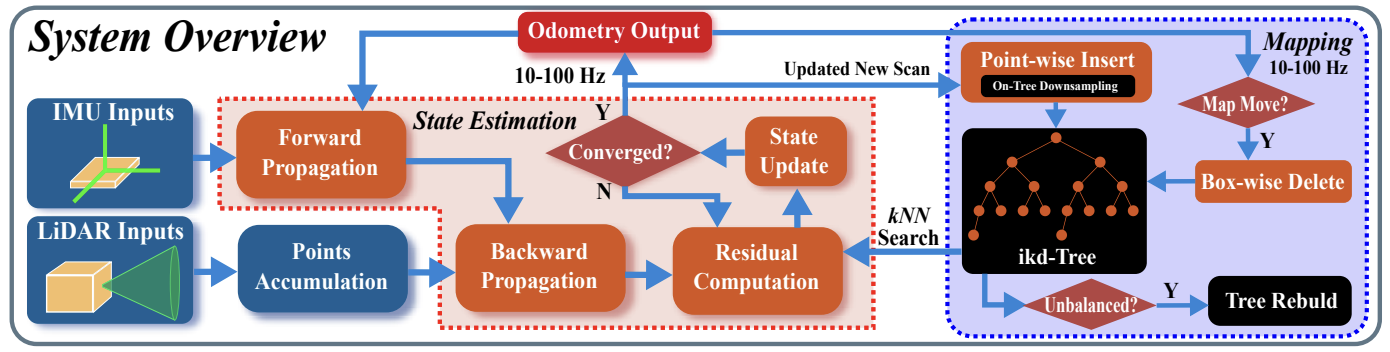
\includegraphics[width=1\textwidth]{gambar/bab2/fast-lio2.png}
    \caption{Diagram sistem \emph{Fast-LIO2}.}
    \label{fig:fastlio2}
    \footnotesize{\textbf{Sumber:} W. Xu et al. (2021)}
\end{figure}

\emph{Fast-LIO2} terbukti unggul dalam 19 sekuen dataset publik dan mampu berjalan hingga 100 Hz, bahkan dalam kondisi ekstrem seperti rotasi hingga $1000^\circ/\text{s}$ \cite{xu2022fastlio}.

\subsubsection{2.2.5.4 Fast-LIO-SAM sebagai Generator Peta}

\emph{Fast-LIO-SAM} adalah pengembangan dari \emph{Fast-LIO2} yang menggabungkan estimasi odometri berbasis \emph{LiDAR-Inertial Odometry} (\emph{LIO}) dengan backend optimisasi graf berbasis \emph{Smoothing and Mapping} (\emph{SAM}). Sistem ini memisahkan proses estimasi pose (\emph{frontend}) dan pemetaan serta koreksi \emph{loop closure (backend)}, sehingga mampu menghasilkan peta 3D yang konsisten dan akurat dalam skala besar. Salah satu keunggulan utama dari \emph{Fast-LIO-SAM} adalah kemampuannya untuk membangun dan menyimpan peta lingkungan dalam format data \texttt{.bag} (ROS bag file). Peta ini berisi informasi spasial hasil integrasi data \emph{LiDAR} dan \emph{IMU} yang telah dioptimasi secara global, dan dapat digunakan kembali untuk proses lokalisasi berulang di waktu yang berbeda tanpa perlu membangun ulang peta. Struktur peta voxel yang digunakan dalam \emph{backend SAM} membuat sistem ini efisien dalam konsumsi memori dan mendukung pemrosesan \emph{real-time}. Oleh karena itu, \emph{Fast-LIO-SAM} ideal digunakan sebagai tahap awal dalam pipeline sistem navigasi otonom, terutama ketika diperlukan peta dasar (\emph{prior map}) untuk aplikasi lokalisasi jangka panjang \cite{xu2022fastlio}.

\subsubsection{2.2.5.5 Fast-LIO Localization QN: Integrasi Quatro dan NanoGICP}

\emph{Fast-LIO Localization QN} adalah sistem lokalisasi berbasis peta yang dirancang untuk bekerja dengan peta hasil dari sistem seperti \emph{Fast-LIO-SAM}. Peta yang telah dibangun dan disimpan dalam format \texttt{.bag} melalui proses SLAM sebelumnya akan digunakan sebagai referensi untuk melakukan lokalisasi kembali terhadap data \emph{LiDAR} baru. Pendekatan ini memungkinkan navigasi yang presisi dan efisien tanpa harus melakukan pemetaan ulang secara terus-menerus.Arsitektur QN menggabungkan modul odometri dari \emph{Fast-LIO2} dengan dua komponen utama dalam proses \emph{map matching}, yaitu \emph{Quatro} dan \emph{NanoGICP}. \emph{Quatro} digunakan untuk melakukan registrasi global cepat, yang memberikan perkiraan awal transformasi posisi sensor terhadap peta. Hal ini sangat penting dalam skenario dengan deviasi posisi awal besar atau ketika sistem baru aktif. Setelah diperoleh transformasi awal, \emph{NanoGICP} digunakan untuk proses refinemen lokal. Algoritma ini merupakan kombinasi dari \emph{FastGICP} dan \emph{NanoFLANN}, yang memungkinkan pencocokan lokal secara presisi tinggi dengan beban komputasi rendah. Integrasi ini memungkinkan proses lokalisasi yang cepat, akurat, dan tahan terhadap noise lingkungan. Karena QN tidak melakukan pemetaan ulang, sistem ini sangat cocok untuk digunakan dalam skenario di mana peta telah tersedia, seperti area industri, fasilitas logistik, gudang, dan bangunan besar dengan struktur tetap. Sistem ini juga mempercepat waktu inisialisasi dan mengurangi konsumsi sumber daya komputasi, karena hanya fokus pada lokalisasi berbasis peta referensi yang diberikan\cite{fastlio2023qnloc}.


\subsection{\emph{Navigation}}
\emph{Path navigation} merupakan komponen kunci dalam sistem robotik bergerak otonom. Komponen ini bertugas memastikan bahwa robot dapat mengikuti jalur yang telah direncanakan sekaligus mampu bereaksi terhadap dinamika lingkungan seperti rintangan statis maupun bergerak. Pendekatan navigasi umumnya dibagi menjadi dua: pengendalian jalur (\emph{path following}) dan penghindaran rintangan (\emph{obstacle avoidance}). Dalam subbagian ini dibahas tiga pendekatan utama yang sering digunakan dan relevan untuk integrasi sistem navigasi cerdas, yaitu \emph{PID controller}, \emph{Braitenberg-based obstacle avoidance}, dan \emph{Pure Pursuit}.

\subsubsection{2.2.6.1 \emph{PID Controller}}

Pengendali PID (\emph{Proportional-Integral-Derivative}) merupakan salah satu algoritma kontrol klasik yang masih luas digunakan karena kesederhanaannya dan efektivitasnya dalam berbagai aplikasi sistem dinamis. PID terdiri dari tiga komponen utama yang bekerja secara sinergis dalam mengurangi kesalahan (\emph{error}) antara nilai keluaran aktual dan nilai referensi sistem. Komponen  \emph{proportional} (\(P\)), memberikan respons sebanding terhadap besarnya \emph{error} saat ini. Semakin besar \emph{error}, semakin besar koreksi yang diberikan, yang membantu sistem mendekati set point secara langsung. Komponen  \emph{integral} (\(I\)), menjumlahkan \emph{error} dari waktu ke waktu untuk mengoreksi kesalahan tetap (\emph{steady-state error}) yang tidak bisa dihilangkan hanya dengan kontrol \emph{proportional}. Komponen \emph{derivative} (\(D\)), bertindak berdasarkan laju perubahan \emph{error}, memberikan peredaman (\emph{damping}) terhadap respons sistem, dan mengurangi gejala \emph{overshoot} serta mempercepat  (\emph{rise time}) menuju \emph{set point}. Secara matematis, sinyal kontrol total \( u(t) \) dalam pengendali PID dapat dirumuskan sebagai:
\begin{equation}
    u(t) = K_p e(t) + K_i \int_{0}^{t} e(\tau) \, d\tau + K_d \frac{d}{dt}e(t),
\end{equation}
di mana \( K_p \), \( K_i \), dan \( K_d \) masing-masing adalah konstanta penguatan (\emph{gain}) untuk komponen \emph{proportional}, \emph{integral}, dan \emph{derivative}, dan \( e(t) \) adalah sinyal kesalahan pada waktu \( t \). Dalam konteks navigasi jalur, pengendali PID umum digunakan untuk mengatur kecepatan linier dan sudut belok robot berdasarkan \emph{cross-track error} (deviasi lateral terhadap jalur) dan \emph{heading error} (perbedaan orientasi). Parameter PID yang dituning dengan baik dapat meminimalkan \emph{steady-state error}, mengontrol \emph{overshoot}, serta mempercepat \emph{rise time} menuju kondisi stabil. Namun, dalam lingkungan yang sangat dinamis atau nonlinear, efektivitas PID dapat menurun karena sifatnya yang tidak adaptif terhadap perubahan konteks \cite{astrom1995pid}.


\subsubsection{2.2.6.2 Braitenberg \emph{Obstacle Avoidance}}

Penghindaran rintangan berdasarkan prinsip \emph{Braitenberg} merupakan pendekatan reaktif yang meniru perilaku biologis sederhana, di mana sensor (misalnya ultrasonik atau LiDAR) dihubungkan langsung ke aktuator secara fungsional. Dalam bentuk dasar, intensitas pembacaan sensor mempengaruhi kecepatan roda secara langsung untuk menghindari objek yang terdeteksi. Meskipun sangat sederhana, pendekatan ini efektif dalam menghindari tabrakan di lingkungan yang tidak terstruktur. Namun, karena sifatnya yang reaktif, metode ini cenderung menghasilkan gerakan tidak halus dan kurang optimal dalam konteks navigasi jalur kompleks. Oleh karena itu, Braitenberg sering digunakan sebagai lapisan reaktif tambahan pada sistem pengendalian berbasis jalur seperti PID atau Pure Pursuit \cite{braitenberg1986vehicles}.

\subsubsection{2.2.6.3 Pure Pursuit untuk Pelacakan Jalur}

\emph{Pure Pursuit} adalah algoritma pelacakan jalur berbasis geometri yang dirancang untuk mengarahkan robot menuju sebuah titik target (\emph{look-ahead point}) yang berada di depan lintasan referensi. Algoritma ini populer karena kesederhanaannya serta kemampuannya menghasilkan lintasan yang halus, terutama pada sistem robotik non-ackermann seperti robot dengan \emph{differential drive}. Prinsip kerja \emph{Pure Pursuit} adalah membentuk lintasan lengkung dari posisi robot menuju titik target. Sudut belok atau kelengkungan lintasan dihitung berdasarkan sudut \( \alpha \), yaitu sudut antara arah heading robot saat ini dan garis lurus ke titik target, serta jarak \emph{look-ahead} \(L_d\). Kelengkungan lintasan ditentukan oleh persamaan:
\begin{equation}
    \kappa = \frac{2 \cdot \sin(\alpha)}{L_d},
\end{equation}
di mana \( \kappa \) kemudian dikonversi menjadi kecepatan sudut:
\begin{equation}
    \omega = v \cdot \kappa,
\end{equation}
dengan \( v \) adalah kecepatan linier robot.

\emph{Look ahed distance} \(L_d\) sangat memengaruhi karakteristik gerakan yang dihasilkan oleh algoritma ini. Ketika nilai \(L_d\) terlalu kecil, robot menjadi sangat responsif terhadap perubahan arah, sehingga sering kali menghasilkan lintasan yang terlalu tajam atau osilatif, terutama pada kecepatan tinggi. Sebaliknya, jika \(L_d\) terlalu besar, robot cenderung mengambil jalur yang lebih lurus dan memotong tikungan, sehingga berpotensi menyimpang dari lintasan referensi. Oleh karena itu, pemilihan nilai \(L_d\) perlu mempertimbangkan kecepatan dan konteks lingkungan. Beberapa implementasi bahkan menggunakan skema adaptif yang menyesuaikan \(L_d\) secara dinamis seiring dengan kecepatan robot untuk menjaga keseimbangan antara stabilitas dan akurasi pelacakan. Metode \emph{Pure Pursuit} sangat cocok untuk navigasi jalur dengan geometri kompleks karena mampu menyesuaikan arah gerak secara kontinu berdasarkan posisi dan heading saat ini. Untuk meningkatkan stabilitas sistem dan mengurangi osilasi gerakan, algoritma ini sering dikombinasikan dengan pengendali PID yang mengatur kecepatan sudut berdasarkan nilai kelengkungan yang dihitung \cite{coulter1992implementation}.


\subsection{\emph{Computer Vision}}

\emph{Computer vision} merupakan cabang dari kecerdasan buatan yang bertujuan untuk memungkinkan komputer memahami dan menganalisis informasi dari citra maupun video digital. Tidak seperti manusia yang secara intuitif dapat mengenali objek, memperkirakan jarak, dan memahami konteks visual, sistem \emph{computer vision} memerlukan algoritma matematis dan pemrograman tingkat lanjut untuk meniru proses tersebut. Salah satu perkembangan penting dalam bidang ini adalah penggunaan arsitektur \emph{Convolutional Neural Network} (CNN), yang menjadi fondasi dalam berbagai aplikasi seperti klasifikasi citra, segmentasi semantik, serta deteksi objek. Salah satu algoritma deteksi objek yang paling populer adalah \emph{You Only Look Once} (YOLO). YOLO telah mengalami banyak peningkatan sejak pertama kali diperkenalkan pada tahun 2016, dengan tujuan untuk meningkatkan kecepatan dan akurasi deteksi objek dalam citra. YOLO bekerja dengan membagi citra menjadi grid dan memprediksi bounding box serta kelas objek dalam satu langkah pemrosesan, menjadikannya sangat efisien untuk aplikasi \emph{real-time}.


\subsubsection{2.2.7.1 YOLOv8}
\emph{YOLOv8} merupakan pengembangan dari algoritma \emph{You Only Look Once} yang menggunakan pendekatan deteksi satu tahap (\emph{one-stage detection}). Model ini mendeteksi objek secara langsung dari keseluruhan citra dalam satu proses, tanpa perlu memisahkannya menjadi beberapa bagian seperti pada metode dua tahap. Peningkatan utama pada \emph{YOLOv8} meliputi optimasi deteksi multi-skala, penggunaan \emph{backbone} yang efisien seperti \emph{CSPDarknet}, serta \emph{neck} yang ditingkatkan untuk ekstraksi fitur, seperti \emph{PANet}. Arsitektur ini memungkinkan deteksi yang cepat dan akurat, serta efisien untuk diterapkan pada perangkat dengan daya komputasi terbatas.  Dengan kombinasi kecepatan, akurasi, dan efisiensi, \emph{YOLOv8} banyak digunakan dalam berbagai aplikasi \emph{computer vision}, termasuk sistem keamanan, kendaraan otonom, dan pengolahan citra medis \cite{yolov8}.


\subsubsection{2.2.7.2 OpenVINO}
OpenVINO (\emph{Open Visual Inference and Neural Network Optimization}) adalah toolkit dari Intel yang dirancang untuk mempercepat inferensi model \emph{deep learning} pada perangkat keras yang berbeda, termasuk CPU, GPU, dan VPU. Dengan menggunakan OpenVINO, model \emph{YOLOv8} dapat dioptimalkan untuk berjalan pada perangkat edge dengan efisiensi tinggi. OpenVINO mendukung berbagai format model, termasuk TensorFlow, PyTorch, dan ONNX, serta menyediakan alat untuk konversi model ke format \emph{Intermediate Representation} (IR) yang lebih efisien. Selain itu, OpenVINO juga menawarkan optimasi presisi data seperti \texttt{FP16} (16-bit floating point) dan \texttt{INT8} (8-bit integer), yang memungkinkan peningkatan performa inferensi dengan kompromi minimal terhadap akurasi. Dengan demikian, OpenVINO sangat cocok untuk aplikasi \emph{real-time} seperti pemantauan suhu termal pada gardu listrik \cite{openvino2021toolkit}.

\subsection{Metode Evaluasi dalam \emph{Computer Vision}}

Evaluasi performa model dalam \emph{computer vision} sangat penting untuk mengukur efektivitas sistem dalam mendeteksi dan mengklasifikasikan objek secara akurat. Beberapa metrik evaluasi yang umum digunakan meliputi \emph{confusion matrix}, \emph{precision}, \emph{recall}, \emph{accuracy}, \emph{F1 score}, dan \emph{loss function}. Masing-masing metrik memberikan perspektif yang berbeda mengenai kinerja model, baik dari segi akurasi keseluruhan, kesalahan klasifikasi, maupun keseimbangan antara kesalahan positif dan negatif.

\subsubsection{2.2.8.1 \emph{Confusion Matrix}}
\emph{Confusion matrix} merupakan sebuah representasi dalam bentuk matriks yang digunakan untuk mengevaluasi kinerja model klasifikasi, khususnya dalam konteks pembelajaran mesin. Matriks ini menunjukkan distribusi hasil prediksi model terhadap data uji, dengan mengklasifikasikan hasil tersebut ke dalam kategori prediksi benar dan salah. Untuk kasus klasifikasi biner, \emph{confusion matrix} terdiri dari empat komponen utama, yaitu \emph{True Positive (TP)}, yang menunjukkan jumlah data positif yang berhasil diklasifikasikan dengan benar; \emph{True Negative (TN)}, yaitu jumlah data negatif yang juga diprediksi dengan tepat; \emph{False Positive (FP)}, yaitu data negatif yang salah diklasifikasikan sebagai positif; serta \emph{False Negative (FN)}, yaitu data positif yang secara keliru diprediksi sebagai negatif.




\begin{figure}[H]
  \centering
  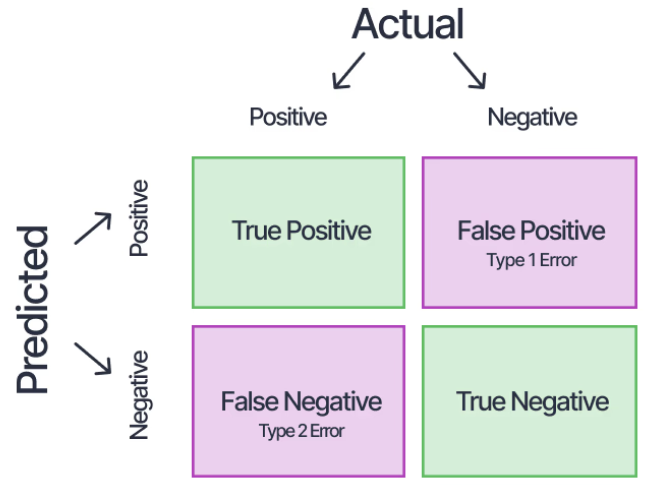
\includegraphics[scale=0.7]{gambar/bab2/cf.png}
  \caption{Contoh \emph{confusion matrix} untuk klasifikasi biner.}
  \label{fig:cf}
  \footnotesize{\textbf{Sumber:} V7Labs (2022)}
\end{figure}

Melalui analisis terhadap keempat komponen ini, pengguna dapat mengevaluasi secara lebih mendalam jenis kesalahan yang terjadi pada model, seperti kecenderungan overfitting terhadap kelas tertentu atau ketidakseimbangan prediksi. Informasi dari \emph{confusion matrix} juga menjadi dasar dalam perhitungan metrik evaluasi lain seperti \emph{accuracy}, \emph{precision}, \emph{recall}, dan \emph{F1-score}, yang lebih menggambarkan performa model secara menyeluruh dalam konteks prediksi klasifikasi.

\subsubsection{A. \emph{Precision}, \emph{Recall}, dan \emph{Accuracy}}

\emph{Precision} menunjukkan seberapa akurat prediksi positif yang dilakukan model, sementara \emph{recall} mengukur seberapa banyak data positif yang berhasil dikenali oleh model. \emph{Accuracy} mengukur persentase keseluruhan prediksi yang benar.

\begin{equation}
  Precision = \frac{TP}{TP + FP}
\end{equation}

\begin{equation}
  Recall = \frac{TP}{TP + FN}
\end{equation}

\begin{equation}
  Accuracy = \frac{TP + TN}{TP + TN + FP + FN}
\end{equation}

\subsubsection{B. \emph{F1 Score}}

\emph{F1 score} adalah rata-rata harmonis antara \emph{precision} dan \emph{recall}. Metrik ini sangat berguna ketika terdapat ketidakseimbangan kelas pada data.

\begin{equation}
  F_1 = 2 \times \frac{Precision \times Recall}{Precision + Recall}
\end{equation}

\subsubsection{C. \emph{Loss Function}}

\emph{Loss function} berfungsi untuk mengukur seberapa jauh prediksi model dari nilai sebenarnya. Fungsi ini digunakan selama pelatihan model untuk meminimalkan kesalahan prediksi. Salah satu fungsi kerugian yang paling umum digunakan dalam klasifikasi adalah \emph{cross-entropy loss}.

\begin{equation}
L = -\sum_{i=1}^{C} y_i \log(p_i)
\end{equation}

Di mana \( C \) adalah jumlah kelas, \( y_i \) adalah label asli untuk kelas ke-\(i\), dan \( p_i \) adalah probabilitas prediksi model terhadap kelas ke-\(i\).


\subsection{\emph{Web GUI}}

\emph{Web Graphical User Interface} atau \emph{Web GUI} merupakan evolusi dari antarmuka pengguna tradisional yang umumnya dijalankan melalui aplikasi desktop. Dengan memanfaatkan teknologi web, \emph{Web GUI} memungkinkan pengguna untuk berinteraksi dengan sistem atau aplikasi melalui peramban web (\emph{browser}) tanpa memerlukan instalasi perangkat lunak tambahan, sehingga memberikan fleksibilitas tinggi dan aksesibilitas yang luas \cite{krug2014dont}. Keunggulan utama dari \emph{Web GUI} dibandingkan dengan GUI konvensional terletak pada sifatnya yang lintas platform dan berbasis cloud. Selama pengguna memiliki koneksi internet dan peramban modern, aplikasi dapat diakses secara langsung tanpa bergantung pada sistem operasi tertentu \cite{murugesan2007web}. Selain itu, proses pemeliharaan dan pembaruan (\emph{update}) menjadi lebih efisien, karena seluruh perubahan dapat dilakukan secara terpusat pada sisi server tanpa perlu mendistribusikan ulang perangkat lunak kepada setiap pengguna. Dalam konteks pengembangan sistem modern, \emph{Web GUI} sangat didukung oleh berbagai teknologi berbasis JavaScript dan framework pendukung yang memungkinkan pengembangan antarmuka yang cepat, responsif, dan \emph{scalable}. 

\subsubsection{2.2.9.1 React.js}

React.js merupakan salah satu \emph{library} \emph{JavaScript} yang umum digunakan dalam pengembangan antarmuka pengguna (\emph{user interface}) yang dinamis dan interaktif. React mengadopsi pendekatan berbasis \emph{component}, yaitu unit antarmuka yang terpisah dan modular, sehingga memudahkan proses pengembangan, pemeliharaan, serta pengujian perangkat lunak. Komponen dalam React dapat dibangun melalui dua pendekatan utama, yaitu \emph{class components} dan \emph{functional components}, yang keduanya bertanggung jawab dalam proses \emph{rendering} elemen antarmuka berdasarkan \emph{props} dan \emph{state} \cite{Panjaitan2021}. Efisiensi dalam pembaruan antarmuka didukung oleh penerapan \emph{Virtual DOM}, yang memungkinkan perubahan hanya terjadi pada bagian yang terdampak tanpa memuat ulang seluruh halaman. Pendekatan ini tidak hanya meningkatkan keterbacaan dan perawatan kode, tetapi juga mendukung prinsip \emph{reusability}, yakni penggunaan kembali komponen di berbagai konteks pengembangan. Dengan karakteristik tersebut, React.js menjadi salah satu teknologi dominan dalam pengembangan aplikasi web berbasis \emph{single-page application} (\emph{SPA}) \cite{Panjaitan2021}.

\subsubsection{2.2.9.2 Next.js}
Next.js merupakan \emph{framework} berbasis \emph{React} yang dikembangkan untuk mendukung pengembangan aplikasi web \emph{full-stack} secara efisien dan terstruktur. Sebagai ekstensi dari \emph{React}, Next.js menyederhanakan berbagai konfigurasi tingkat rendah seperti \emph{module bundling}, \emph{routing}, dan \emph{code splitting}, yang umumnya memerlukan pengaturan manual dalam proyek \emph{React} murni \cite{Nextjs2024}. Kemampuan ini memungkinkan pengembang untuk fokus pada pengembangan fitur tanpa harus terlibat langsung dalam proses pengelolaan infrastruktur aplikasi. Next.js mengintegrasikan secara native pendekatan \emph{server-side rendering} (SSR) dan \emph{static site generation} (SSG), dua teknik rendering yang krusial dalam optimalisasi performa dan aksesibilitas halaman web. SSR memungkinkan halaman dirender di sisi server sebelum dikirim ke klien, sehingga mengurangi waktu muat awal pada web browswer. Di sisi lain, SSG menghasilkan halaman statis pada waktu kompilasi, yang secara signifikan menurunkan beban server dan mempercepat distribusi konten. Kombinasi kedua pendekatan ini memberikan fleksibilitas tinggi dalam strategi rendering berdasarkan kebutuhan spesifik aplikasi. Dalam konteks pengembangan berbasis komponen, integrasi React dan Next.js mendukung pengembangan antarmuka interaktif dengan performa tinggi. Studi mutakhir menunjukkan bahwa implementasi \emph{framework} seperti Next.js dapat menurunkan latensi interaksi, meningkatkan \emph{user engagement}, serta mendukung skalabilitas dalam arsitektur perangkat lunak modern \cite{Nextjs2024}.

\subsubsection{2.2.9.3 Tailwind CSS}

Tailwind CSS merupakan \emph{framework} \emph{utility-first} berbasis CSS yang mengedepankan penggunaan kelas utilitas langsung dalam markup untuk membentuk antarmuka pengguna yang responsif dan terstruktur. Berbeda dengan \emph{framework} tradisional yang menyediakan komponen siap pakai, pendekatan Tailwind memungkinkan fleksibilitas tinggi dan iterasi cepat dalam pengembangan desain kustom \cite{Azhariyah2024}. Integrasinya yang seamless dengan \emph{framework} JavaScript seperti React dan Angular memperkuat efisiensi pengembangan berbasis komponen, sekaligus mengurangi kebutuhan akan file CSS yang besar. Dukungan bawaan terhadap desain responsif menjadikan Tailwind CSS relevan untuk pengembangan aplikasi lintas perangkat dengan konsistensi visual yang tinggi.

\subsubsection{2.2.9.4 ShadCN}

ShadCN UI merupakan kumpulan komponen \emph{React} modern yang bersifat \emph{open-source}, namun tidak dikemas sebagai pustaka tradisional yang dapat diinstal melalui \emph{Node Package Manager} (\emph{npm}). Sebaliknya, pengembang menyalin langsung kode sumber komponen ke dalam basis kode proyek, sehingga memberikan fleksibilitas tinggi dalam modifikasi fungsionalitas dan penataan. Komponen-komponen ini menggunakan \emph{Tailwind CSS} untuk styling, dengan desain awal yang konsisten dan minimalis. ShadCN menyediakan beragam komponen antarmuka umum seperti \emph{dialog}, \emph{input}, \emph{checkbox}, dan \emph{table}, serta mendukung integrasi cepat melalui perintah \emph{CLI} untuk menyalin kode ke dalam direktori lokal proyek \cite{Shadcn2024}. Pendekatan ini menghasilkan aplikasi yang lebih ringan dan modular, karena hanya menyertakan komponen yang benar-benar dibutuhkan.

\subsubsection{2.2.9.4 Express.js}
Express.js adalah \emph{framework} minimalis untuk Node.js yang dirancang untuk membangun aplikasi web dan API dengan cepat dan efisien. Dengan arsitektur yang sederhana dan fleksibel, Express memungkinkan pengembang untuk membuat aplikasi dengan struktur yang jelas dan mudah dipelihara. Salah satu fitur utama dari Express adalah kemampuannya untuk menangani berbagai jenis permintaan HTTP, serta mendukung middleware yang memungkinkan penanganan permintaan secara modular. Middleware ini dapat digunakan untuk berbagai tujuan, seperti otentikasi, pengolahan data, dan penanganan kesalahan \cite{express2023docs}. Selain itu, Express juga memiliki ekosistem yang luas dengan banyak pustaka tambahan yang dapat diintegrasikan untuk memperluas fungsionalitas aplikasi. Dengan demikian, Express.js menjadi pilihan populer bagi pengembang yang ingin membangun aplikasi web modern dengan cepat dan efisien.

\subsubsection{2.2.9.5 PostgreSQL}
PostgreSQL, sebuah sistem manajemen basis data relasional (RDBMS) \emph{open-source} yang terkenal, telah menjadi pilihan utama dalam pengembangan aplikasi berbasis data. Dengan arsitektur yang kuat dan dukungan untuk berbagai fitur, PostgreSQL menawarkan kemampuan yang sangat baik dalam hal penyimpanan, pengambilan, dan manipulasi data. Sistem ini dikenal karena kepatuhannya terhadap standar SQL, serta kemampuannya untuk menangani transaksi kompleks dengan tingkat konsistensi yang tinggi \cite{postgresql2023docs}. PostgreSQL juga mendukung berbagai tipe data, termasuk JSON dan XML, yang memungkinkan fleksibilitas dalam menyimpan data semi-terstruktur dan tidak terstruktur. Selain itu, sistem ini memiliki ekosistem yang kaya dengan banyak ekstensi dan modul tambahan yang dapat meningkatkan fungsionalitasnya lebih lanjut \cite{postgresql2023docs}.


\subsubsection{2.2.9.6 WebSocket}
WebSocket adalah protokol komunikasi dua arah yang beroperasi di atas koneksi TCP yang persisten, memungkinkan pertukaran pesan antara klien dan server secara efisien. Protokol ini dirancang untuk mengatasi kekurangan teknologi komunikasi dua arah yang ada sebelumnya, yang sering menggunakan \emph{HTTP} sebagai lapisan transportasi. Dengan memanfaatkan mekanisme \emph{upgrade} dari \emph{HTTP}, WebSocket dapat membuka saluran komunikasi bidirectional yang lebih efisien dibandingkan dengan pendekatan tradisional seperti \emph{polling} atau \emph{long polling} \cite{Fette2011}. Keunggulan utama dari WebSocket terletak pada kemampuannya untuk mengurangi overhead komunikasi, yang sangat penting dalam aplikasi yang memerlukan pembaruan real-time, seperti aplikasi \emph{chat}, permainan daring, dan sistem \emph{IoT}. Penelitian menunjukkan bahwa WebSocket tidak hanya meningkatkan efisiensi komunikasi, tetapi juga memungkinkan pengembangan aplikasi kolaboratif yang lebih responsif dan interaktif \cite{Milsap2019}. Dengan demikian, WebSocket menjadi solusi yang ideal untuk aplikasi yang membutuhkan latensi rendah dan kecepatan tinggi dalam pertukaran data.


